\documentclass[a4paper]{article}

\def\npart {IB}
\def\nterm {Lent}
\def\nyear {2016}
\def\nlecturer {I. Smith}
\def\ncourse {Complex Analysis}
\def\nlectures {MWF.11}
\def\nnotready {}

% Imports
\ifx \nextra \undefined
  \usepackage[pdftex,
    hidelinks,
    pdfauthor={Dexter Chua},
    pdfsubject={Cambridge Maths Notes: Part \npart\ - \ncourse},
    pdftitle={Part \npart\ - \ncourse},
  pdfkeywords={Cambridge Mathematics Maths Math \npart\ \nterm\ \nyear\ \ncourse}]{hyperref}
  \title{Part \npart\ - \ncourse}
\else
  \usepackage[pdftex,
    hidelinks,
    pdfauthor={Dexter Chua},
    pdfsubject={Cambridge Maths Notes: Part \npart\ - \ncourse\ (\nextra)},
    pdftitle={Part \npart\ - \ncourse\ (\nextra)},
  pdfkeywords={Cambridge Mathematics Maths Math \npart\ \nterm\ \nyear\ \ncourse\ \nextra}]{hyperref}

  \title{Part \npart\ - \ncourse \\ {\Large \nextra}}
\fi

\author{Lectured by \nlecturer \\\small Notes taken by Dexter Chua}
\date{\nterm\ \nyear}

\usepackage{alltt}
\usepackage{amsfonts}
\usepackage{amsmath}
\usepackage{amssymb}
\usepackage{amsthm}
\usepackage{booktabs}
\usepackage{caption}
\usepackage{enumitem}
\usepackage{fancyhdr}
\usepackage{graphicx}
\usepackage{mathtools}
\usepackage{microtype}
\usepackage{multirow}
\usepackage{pdflscape}
\usepackage{pgfplots}
\usepackage{siunitx}
\usepackage{tabularx}
\usepackage{tikz}
\usepackage{tkz-euclide}
\usepackage[normalem]{ulem}
\usepackage[all]{xy}

\pgfplotsset{compat=1.12}

\pagestyle{fancyplain}
\lhead{\emph{\nouppercase{\leftmark}}}
\ifx \nextra \undefined
  \rhead{
    \ifnum\thepage=1
    \else
      \npart\ \ncourse
    \fi}
\else
  \rhead{
    \ifnum\thepage=1
    \else
      \npart\ \ncourse\ (\nextra)
    \fi}
\fi
\usetikzlibrary{arrows}
\usetikzlibrary{decorations.markings}
\usetikzlibrary{decorations.pathmorphing}
\usetikzlibrary{positioning}
\usetikzlibrary{fadings}
\usetikzlibrary{intersections}
\usetikzlibrary{cd}

\newcommand*{\Cdot}{\raisebox{-0.25ex}{\scalebox{1.5}{$\cdot$}}}
\newcommand {\pd}[2][ ]{
  \ifx #1 { }
    \frac{\partial}{\partial #2}
  \else
    \frac{\partial^{#1}}{\partial #2^{#1}}
  \fi
}

% Theorems
\theoremstyle{definition}
\newtheorem*{aim}{Aim}
\newtheorem*{axiom}{Axiom}
\newtheorem*{claim}{Claim}
\newtheorem*{cor}{Corollary}
\newtheorem*{defi}{Definition}
\newtheorem*{eg}{Example}
\newtheorem*{fact}{Fact}
\newtheorem*{law}{Law}
\newtheorem*{lemma}{Lemma}
\newtheorem*{notation}{Notation}
\newtheorem*{prop}{Proposition}
\newtheorem*{thm}{Theorem}

\renewcommand{\labelitemi}{--}
\renewcommand{\labelitemii}{$\circ$}
\renewcommand{\labelenumi}{(\roman{*})}

\let\stdsection\section
\renewcommand\section{\newpage\stdsection}

% Strike through
\def\st{\bgroup \ULdepth=-.55ex \ULset}

% Maths symbols
\newcommand{\bra}{\langle}
\newcommand{\ket}{\rangle}

\newcommand{\N}{\mathbb{N}}
\newcommand{\Z}{\mathbb{Z}}
\newcommand{\Q}{\mathbb{Q}}
\renewcommand{\H}{\mathbb{H}}
\newcommand{\R}{\mathbb{R}}
\newcommand{\C}{\mathbb{C}}
\newcommand{\Prob}{\mathbb{P}}
\renewcommand{\P}{\mathbb{P}}
\newcommand{\E}{\mathbb{E}}
\newcommand{\F}{\mathbb{F}}
\newcommand{\cU}{\mathcal{U}}
\newcommand{\RP}{\mathbb{RP}}
\newcommand{\CP}{\mathbb{CP}}

\newcommand{\ph}{\,\cdot\,}

\DeclareMathOperator{\sech}{sech}
\DeclareMathOperator{\cosech}{cosech}
\DeclareMathOperator{\cosec}{cosec}

\DeclareMathOperator{\covol}{covol}
\DeclareMathOperator{\vol}{vol}

\let\Im\relax
\let\Re\relax
\DeclareMathOperator{\Im}{Im}
\DeclareMathOperator{\Re}{Re}
\DeclareMathOperator{\im}{im}
\DeclareMathOperator{\image}{image}
\DeclareMathOperator{\Ann}{Ann}

\DeclareMathOperator*{\res}{res}
\DeclareMathOperator{\Res}{Res}
\DeclareMathOperator{\Ind}{Ind}

\DeclareMathOperator{\tr}{tr}
\DeclareMathOperator{\diag}{diag}
\DeclareMathOperator{\rank}{rank}
\DeclareMathOperator{\card}{card}
\DeclareMathOperator{\spn}{span}
\DeclareMathOperator{\adj}{adj}

\DeclareMathOperator{\erf}{erf}
\DeclareMathOperator{\erfc}{erfc}

\DeclareMathOperator{\ord}{ord}
\DeclareMathOperator{\Sym}{Sym}

\DeclareMathOperator{\sgn}{sgn}
\DeclareMathOperator{\orb}{orb}
\DeclareMathOperator{\stab}{stab}
\DeclareMathOperator{\ccl}{ccl}

\DeclareMathOperator{\lcm}{lcm}
\DeclareMathOperator{\hcf}{hcf}

\DeclareMathOperator{\Int}{Int}
\DeclareMathOperator{\id}{id}

\DeclareMathOperator{\betaD}{beta}
\DeclareMathOperator{\gammaD}{gamma}
\DeclareMathOperator{\Poisson}{Poisson}
\DeclareMathOperator{\binomial}{binomial}
\DeclareMathOperator{\multinomial}{multinomial}
\DeclareMathOperator{\Bernoulli}{Bernoulli}
\DeclareMathOperator{\like}{like}

\DeclareMathOperator{\var}{var}
\DeclareMathOperator{\cov}{cov}
\DeclareMathOperator{\bias}{bias}
\DeclareMathOperator{\mse}{mse}
\DeclareMathOperator{\corr}{corr}

\DeclareMathOperator{\otp}{otp}
\DeclareMathOperator{\dom}{dom}

\DeclareMathOperator{\Root}{Root}
\DeclareMathOperator{\supp}{supp}
\DeclareMathOperator{\rel}{rel}
\DeclareMathOperator{\Hom}{Hom}
\DeclareMathOperator{\Aut}{Aut}
\DeclareMathOperator{\Gal}{Gal}
\DeclareMathOperator{\Mat}{Mat}
\DeclareMathOperator{\End}{End}
\DeclareMathOperator{\Char}{char}
\DeclareMathOperator{\ev}{ev}
\DeclareMathOperator{\St}{St}
\DeclareMathOperator{\Lk}{Lk}
\DeclareMathOperator{\disc}{disc}
\DeclareMathOperator{\Isom}{Isom}
\DeclareMathOperator{\length}{length}
\DeclareMathOperator{\energy}{energy}
\DeclareMathOperator{\area}{area}
\DeclareMathOperator{\Syl}{Syl}
\DeclareMathOperator{\cl}{cl}
\DeclareMathOperator{\fix}{fix}

\newcommand{\GL}{\mathrm{GL}}
\newcommand{\SL}{\mathrm{SL}}
\newcommand{\PGL}{\mathrm{PGL}}
\newcommand{\PSL}{\mathrm{PSL}}
\newcommand{\PSU}{\mathrm{PSU}}
\newcommand{\Or}{\mathrm{O}}
\newcommand{\SO}{\mathrm{SO}}
\newcommand{\U}{\mathrm{U}}
\newcommand{\SU}{\mathrm{SU}}

\renewcommand{\d}{\mathrm{d}}
\newcommand{\D}{\mathrm{D}}

\tikzset{->/.style = {decoration={markings,
                                  mark=at position 1 with {\arrow[scale=2]{latex'}}},
                      postaction={decorate}}}
\tikzset{<-/.style = {decoration={markings,
                                  mark=at position 0 with {\arrowreversed[scale=2]{latex'}}},
                      postaction={decorate}}}
\tikzset{<->/.style = {decoration={markings,
                                   mark=at position 0 with {\arrowreversed[scale=2]{latex'}},
                                   mark=at position 1 with {\arrow[scale=2]{latex'}}},
                       postaction={decorate}}}
\tikzset{->-/.style = {decoration={markings,
                                   mark=at position #1 with {\arrow[scale=2]{latex'}}},
                       postaction={decorate}}}
\tikzset{-<-/.style = {decoration={markings,
                                   mark=at position #1 with {\arrowreversed[scale=2]{latex'}}},
                       postaction={decorate}}}

\tikzset{circ/.style = {fill, circle, inner sep = 0, minimum size = 3}}
\tikzset{mstate/.style={circle, draw, blue, text=black, minimum width=0.7cm}}

\definecolor{mblue}{rgb}{0.2, 0.3, 0.8}
\definecolor{morange}{rgb}{1, 0.5, 0}
\definecolor{mgreen}{rgb}{0.1, 0.4, 0.2}
\definecolor{mred}{rgb}{0.5, 0, 0}

\def\drawcirculararc(#1,#2)(#3,#4)(#5,#6){%
    \pgfmathsetmacro\cA{(#1*#1+#2*#2-#3*#3-#4*#4)/2}%
    \pgfmathsetmacro\cB{(#1*#1+#2*#2-#5*#5-#6*#6)/2}%
    \pgfmathsetmacro\cy{(\cB*(#1-#3)-\cA*(#1-#5))/%
                        ((#2-#6)*(#1-#3)-(#2-#4)*(#1-#5))}%
    \pgfmathsetmacro\cx{(\cA-\cy*(#2-#4))/(#1-#3)}%
    \pgfmathsetmacro\cr{sqrt((#1-\cx)*(#1-\cx)+(#2-\cy)*(#2-\cy))}%
    \pgfmathsetmacro\cA{atan2(#2-\cy,#1-\cx)}%
    \pgfmathsetmacro\cB{atan2(#6-\cy,#5-\cx)}%
    \pgfmathparse{\cB<\cA}%
    \ifnum\pgfmathresult=1
        \pgfmathsetmacro\cB{\cB+360}%
    \fi
    \draw (#1,#2) arc (\cA:\cB:\cr);%
}
\newcommand\getCoord[3]{\newdimen{#1}\newdimen{#2}\pgfextractx{#1}{\pgfpointanchor{#3}{center}}\pgfextracty{#2}{\pgfpointanchor{#3}{center}}}

\def\Xint#1{\mathchoice
   {\XXint\displaystyle\textstyle{#1}}%
   {\XXint\textstyle\scriptstyle{#1}}%
   {\XXint\scriptstyle\scriptscriptstyle{#1}}%
   {\XXint\scriptscriptstyle\scriptscriptstyle{#1}}%
   \!\int}
\def\XXint#1#2#3{{\setbox0=\hbox{$#1{#2#3}{\int}$}
     \vcenter{\hbox{$#2#3$}}\kern-.5\wd0}}
\def\ddashint{\Xint=}
\def\dashint{\Xint-}


\begin{document}
\maketitle
{\small
\noindent\textbf{Analytic functions}\\
Complex differentiation and the Cauchy-Riemann equations. Examples. Conformal mappings. Informal discussion of branch points, examples of $\log z$ and $z^c$.\hspace*{\fill} [3]

\vspace{10pt}
\noindent\textbf{Contour integration and Cauchy's theorem}\\
Contour integration (for piecewise continuously differentiable curves). Statement and proof of Cauchy's theorem for star domains. Cauchy's integral formula, maximum modulus theorem, Liouville's theorem, fundamental theorem of algebra. Morera's theorem.\hspace*{\fill} [5]

\vspace{10pt}
\noindent\textbf{Expansions and singularities}\\
Uniform convergence of analytic functions; local uniform convergence. Differentiability of a power series. Taylor and Laurent expansions. Principle of isolated zeros. Residue at an isolated singularity. Classification of isolated singularities.\hspace*{\fill} [4]

\vspace{10pt}
\noindent\textbf{The residue theorem}\\
Winding numbers. Residue theorem. Jordan's lemma. Evaluation of definite integrals by contour integration. Rouch\'es theorem, principle of the argument. Open mapping theorem.\hspace*{\fill} [4]}

\tableofcontents
\section{Complex differentiation}
\subsection{Differentiation}
We first recall a few basic definitions. We are going to look at functions defined on subsets of the complex plane. Often, we just want to look at open subsets.
\begin{defi}[Open subset]
  A subset $U \subseteq \C$ is \emph{open} if for any $x \in U$, there is some $\varepsilon > 0$ such that the open ball $B_x(\varepsilon) = B(x; \varepsilon) \subseteq U$.
\end{defi}
The notation used for the open ball varies form time to time, even within the same sentence. For example, instead of putting $x$ as the subscript, we could put $\varepsilon$ as the subscript and $x$ inside the brackets. Hopefully, it will be clear from context.

\begin{defi}[Path-connected subset]
  A subset $U \subseteq \C$ is path-connected if for any $x, y \in U$, there is some $\gamma: [0, 1] \to U$ continuous such that $\gamma(0) = x$ and $\gamma(1) = y$.
\end{defi}

\begin{defi}[Domain]
  A \emph{domain} is a non-empty open path-connected subset of $\C$.
\end{defi}

Consider a domain $U \subseteq \C$ and a function $f: U \to \C$.
\begin{defi}[Differentiable function]
  We say a function $f$ is \emph{differentiable} at $w \in U$ if
  \[
    f'(w) = \lim_{z\to w} \frac{f(z) - f(w)}{z - w}
  \]
  exists.
\end{defi}
Here we implicitly require that the limit does not depend on which direction we approach $w$ from. It turns out this is a very strong condition to impose.

\begin{defi}[Analytic/holomorphic function]
  A function $f$ is \emph{analytic} or \emph{holomorphic} at $w \in U$ if $f$ is differentiable on an open neighbourhood $B(w, \varepsilon)$ of $w$.
\end{defi}

\begin{defi}[Entire function]
  If $f: \C \to \C$ is defined on all of $\C$ and is holomorphic on $\C$, then $f$ is said to be \emph{entire}.
\end{defi}

The goal of the course is to develop the rich theory of these complex differentiable functions and see how we can integrate them along continuously differentiable ($C^1$) paths in the complex plane.

First, we want to figure out when a function is differentiable. Given $f: U \to \C$, we can write it as $f = u + iv$, where $u, v: U \to \R$ are real-valued functions. Recall from IB Analysis II that a function $u: U \to \R$ viewed as a real-valued function of two variables is differentiable at a point $(c, d) \in U$, with derivative $Du|_{(c, d)} = (\lambda, \mu)$, if and only if
\[
  \frac{u(x, y) - u(c, d) - (\lambda (x - c) + \mu (y - d))}{\|(x, y) - (c, d)\|} \to 0
\]
as $(x, y) \to (c, d)$.

This allows us to come up with a nice criterion for when a function is differentiable
\begin{prop}
  Let $f$ be defined on an open set $U \subseteq \C$. Let $w = c + id \in U$ and write $f = u + iv$. Then $f$ is complex differentiable at $w$ if and only if $u$ and $v$ are differentiable at $(c, d)$, viewed as a real function of two real variables, \emph{and}
  \begin{align*}
    u_x &= v_y\\
    u_y &= -v_x
  \end{align*}
  These equations are the \emph{Cauchy-Riemann equations}. In this case, we have
  \[
    f'(w) = u_x(c, d) + iv_x(c, d) = v_y(c, d) -i u_y(c, d).
  \]
\end{prop}

\begin{proof}
  By definition, $f$ is differentiable at $w$ with $f'(w) = p + iq$ if and only if
  \[
    \lim_{z \to w} \frac{f(z) - f(w) - f'(w)(z - w)}{z - w} = 0. \tag{$\dagger$}
  \]
  If $z = x + iy$, then
  \[
    f'(w) (z - w) = p(x - c) - q(y - d) + i(q(x - c) + p (y - c)).
  \]
  So $(\dagger)$ holds if and only if
  \[
    \lim_{(x, y) \to (c, d)} \frac{u(x, y) - u(c, d) - (p(x - c) - q(y - d))}{\sqrt{(x - c)^2 + (y - d)^2}} = 0
  \]
  and
  \[
    \lim_{(x, y) \to (c, d)} \frac{v(x, y) - v(c, d) - (q(x - c) + p(y - d))}{\sqrt{(x - c)^2 + (y - d)^2}} = 0.
  \]
  Comparing this to the definition of the differentiability of a real-valued function, we see this holds exactly if $u$ and $v$ are differentiable at $(c, d)$ with
  \[
    Du|_{(c, d)} = (p, -q),\quad Dv|_{(c, d)} = (q, p).
  \]
\end{proof}
A standard warning is given that $f: U \to \C$ can be written as $f = u + iv$, where $u_x = v_y$ and $u_y = -v_x$ at $(c, d) \in U$, we \emph{cannot} conclude that $f$ is complex differentiable at $(c, d)$. These conditions only say the partial derivatives exist, but this does \emph{not} imply imply that $u$ and $v$ are differentiable, as required by the proposition. However, if the partial derivatives exist and are continuous, then by IB Analysis II we know they are differentiable.

\begin{eg}\leavevmode
  \begin{enumerate}
    \item A polynomial $p: \C \to \C$ is entire. This can be checked directly from definition.
    \item A \emph{rational function} $\frac{p(z)}{q(z)}: U \to \C$, where $U \subseteq \C \setminus \{z: q(z) = 0\}$, is holomorphic on any such $U$. Here $p, q$ are polynomials.
    \item $f(z) = |z|$ is \emph{not} complex differentiable at \emph{any} point of $\C$. Indeed, we can write this as $f = u + iv$, where
      \[
        u(x, y) = \sqrt{x^2 + y^2},\quad v(x, y) = 0.
      \]
      If $(x, y) \not= (0, 0)$, then
      \[
        u_x = \frac{x}{\sqrt{x^2 + y^2}},\quad u_y = \frac{y}{\sqrt{x^2 + y^2}}.
      \]
      If we are not at the origin, then clearly both cannot vanish, but the partials of $v$ both vanish. Hence the Cauchy-Riemann equations do not hold and it is not differentiable outside of the origin.

      At the origin, we can compute directly that
      \[
        \frac{f(h) - f(0)}{h} = \frac{|h|}{h}.
      \]
      This is, say, $+1$ for $h \in \R^+$ and $-1$ for $h \in \R^-$. So the limit as $h \to 0$ does not exists.
  \end{enumerate}
\end{eg}

\subsection{Conformal mappings}
The course schedules has a weird part where we are supposed to talk about conformal mappings for a lecture, but not use it anywhere else. We have to put them \emph{somewhere}, and we might as well do it now. However, this section will be slightly disconnected from the rest of the lectures.

\begin{defi}[Conformal function]
  Let $f: U \to \C$ be a function holomorphic at $w \in U$. If $f'(w) \not= 0$, we say $f$ is \emph{conformal}.
\end{defi}

Note that if $f = u + iv$, then viewed as a map $\R^2 \to \R^2$, we find the Jacobian matrix is
\[
  Df =
  \begin{pmatrix}
    u_x & u_y\\
    v_x & v_y
  \end{pmatrix}
\]
Then
\[
  \det (Df) = u_x v_y + u_y v_x = u_x^2 + u_y^2.
\]
Using the formula for the complex derivative in terms of the partials, this shows that if $f'(w) \not= 0$, then $\det(Df|_w) \not= 0$. Hence, by the inverse function theorem (viewing $f$ as a function $\R^2 \to \R^2$), $f$ is locally invertible at $w$.

It is an exercise to show that the usual rules of differentiation (sum, product, chain rule, derivative of inverse function) all hold for complex differentiation just as in the real case, with exactly the same proof. In particular, if a holomorphic function is conformal at a point $w$, then it has a local inverse which is also holomorphic and conformal.

Another useful property of conformal mappings is that they preserve angles. To give a precise statement of this, we need to specify how ``angles'' work.

The idea is to look at tangent vectors of paths. Let $\gamma_1, \gamma_2: [-1, 1] \to U$ be continuously differentiable paths that intersect when $t = 0$ at $w = \gamma_1(0) = \gamma_2(0)$. Moreover, assume $\gamma_i'(0) \not= 0$.

Then we can compare the angles between the paths by looking at the difference in arguments of the tangents at $w$. In particular, we define
\[
  \mathrm{angle} (\gamma_1, \gamma_2) = \arg (\gamma_1'(0)) - \arg (\gamma_2'(0)).
\]
(here we take $\arg$ to be the argument we would have if $w$ were the origin)

Let $f: U \to \C$ and $w \in U$. Suppose $f$ is conformal at $w$. Then $f$ maps our two paths to $f \circ \gamma_i: [-1, 1] \to \C$. These two paths now intersect at $f(w)$. Then the angle between them is
\begin{align*}
  \mathrm{angle} (f \circ \gamma_1, f\circ \gamma_2) &= \arg((f\circ \gamma_1)'(0)) - \arg((f \circ \gamma_2)'(0))\\
  &= \arg\left(\frac{(f\circ \gamma_1)'(0)}{(f \circ \gamma_2)'(0)}\right)\\
  &= \arg\left(\frac{\gamma_1'(0)}{\gamma_2'(0)}\right)\\
  &= \mathrm{angle} (\gamma_1, \gamma_2),
\end{align*}
using the chain rule and the fact that $f'(w) \not= 0$.

What the word ``conformal'' really should mean is that it preserves angles. However, we adopt the definition of having non-zero derivative because it is easier to state and check.

We will later prove that if $f: U \to \C$ is holomorphic on an open set $U$, then $f': U \to \C$ is \emph{also} holomorphic. Hence $f$ is infinitely differentiable.

Moreover, if we write $f = u + iv$, then using the formula for $f'$ in terms of the partials, we know $u$ and $v$ are also \emph{infinitely differentiable}. Differentiating the Cauchy-Riemann equations, we get
\[
  u_{xx} = v_{yx} = -u_{yy}.
\]
In other words,
\[
  u_{xx} + u_{yy} = 0,
\]
We get similar results for $v$ instead. Hence $\Re(f)$ and $\Im(f)$ satisfy the Laplace equation and are hence \emph{harmonic} (by definition).

\begin{defi}[Conformal equivalence]
  If $U$ and $V$ are open subsets of $\C$ and $f: U \to V$ is a conformal bijection, then it is a \emph{conformal equivalence}.
\end{defi}
Note that in general, a bijective continuous map need not have a continuous inverse. However, if we are given further that it is \emph{conformal}, then the inverse mapping theorem tells us there is a local conformal inverse, and if the function is bijective, these patch together to give a global conformal inverse.

\begin{eg}
  Any M\"obius map $A(z) = \frac{az + b}{cz + d}$ (with $ad - bc \not= 0$) defines a conformal equivalence $\C \cup \{\infty\} \to \C\cup \{\infty\}$ in the obvious sense. $A'(z) \not= 0$ follows from the chain rule and the invertibility of $A(z)$.

  In particular, the M\"obius group of the disk
  \begin{align*}
    \text{M\"ob}(D) &= \{f \in \text{M\"obius group}: f(D) = D\} \\
    &= \left\{\frac{az + b}{\bar{b}z + \bar{a}} \in \text{M\"ob} : |a|^2 - |b|^2 = 1\right\}
  \end{align*}
  is a group of conformal equivalences of the disk.
\end{eg}
\begin{eg}
  The map $z \mapsto z^n$ for $n \geq 2$ is holomorphic everywhere and conformal except at $z = 0$. This gives a conformal equivalence
  \[
    \left\{z \in \C^*: 0 < \arg(z) < \frac{\pi}{n}\right\} \leftrightarrow \H,
  \]
  where we adopt the following notation:
\end{eg}

\begin{notation}
  We write $\C^* = \C \setminus \{0\}$ and
  \[
    \H = \{z \in \C: \Im (z) > 0\}
  \]
  is the upper half plane.
\end{notation}

\begin{eg}
  Note that $z \in \H$ if and only if $z$ is closer to $i$ than to $-i$. In other words,
  \[
    |z - i| < |z + i|,
  \]
  or
  \[
    \left|\frac{z - i}{z + i}\right| < 1.
  \]
  So $z \mapsto \frac{z - i}{z + i}$ defines a conformal equivalence $\H \to D$, the unit disc. We know this is conformal since it is a special case of the M\"obius map.
\end{eg}

\begin{eg}
  Consider the map
  \[
    z \mapsto w = \frac{1}{2}\left(z + \frac{1}{z}\right),
  \]
  assuming $z \in \C^*$. This can also be written as
  \[
    \frac{w + 1}{w - 1} = 1 + \frac{2}{w - 1} = 1 + \frac{4}{z + \frac{1}{z} - 2} = 1 + \frac{4z}{z^2 - 2z + 1} = \left(\frac{z + 1}{z - 1}\right)^2.
  \]
  So this is just squaring in some funny coordinates given by $\frac{z + 1}{z - 1}$. This map is holomorphic (except at $z = 0$). Also, we have
  \[
    f'(z) = 1 - \frac{z^2 + 1}{2z^2}.
  \]
  So $f$ is conformal except at $\pm 1$.

  Recall that the first thing we learnt about M\"obius maps is that they take lines and circles to lines and circles. This does something different. We write $z = re^{i\theta}$. Then if we write $z \mapsto w = u + iv$, we have
  \begin{align*}
    u &= \frac{1}{2}\left(r + \frac{1}{r}\right) \cos \theta\\
    v &= \frac{1}{2}\left(r - \frac{1}{r}\right) \sin \theta
  \end{align*}
  Fixing the radius and argument fixed respectively, we see that a circle of radius $\rho$ is mapped to the ellipse
  \[
    \frac{u^2}{\frac{1}{4}\left(\rho + \frac{1}{\rho}\right)^2} + \frac{v^2}{\frac{1}{4}\left(\rho - \frac{1}{\rho}\right)^2} = 1,
  \]
  while the half-line $\arg(z) = \mu$ is mapped to the hyperbola
  \[
    \frac{u^2}{\cos^2\mu} - \frac{v^2}{\sin^2 \mu} = 1.
  \]
  We can do something more interesting. Consider a off-centered circle, chosen to pass through the point $-1$ and $-i$. Then the image looks like this:
  \begin{center}
    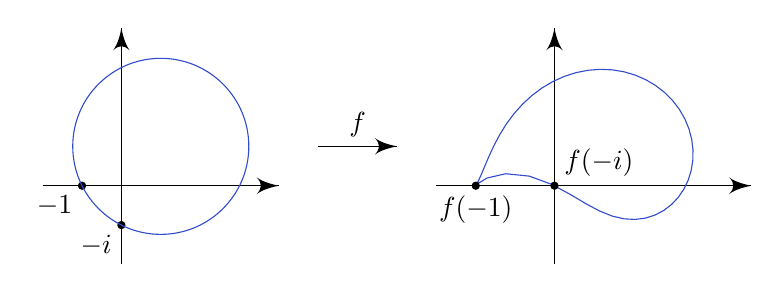
\begin{tikzpicture}[scale=0.5]
      \draw [->] (-2, 0) -- (4, 0);
      \draw [->] (0, -2) -- (0, 4);
      \node [circ] at (-1, 0) {};
      \node [circ] at (0, -1) {};
      \node at (-1, 0) [anchor = north east] {$-1$};
      \node at (0, -1) [anchor = north east] {$-i$};
      \draw [mblue] (1, 1) circle [radius=2.236];

      \draw [->] (5, 1) -- (7, 1) node [pos=0.5, above] {$f$};

      \begin{scope}[shift={(11, 0)}]
        \draw [->] (-3, 0) -- (5, 0);
        \draw [->] (0, -2) -- (0, 4);
        \draw [mblue, domain=0:360, samples=50] plot ({(sqrt (7 + 4.4721*(sin(\x) + cos(\x))) + 1/(sqrt (7 + 4.4721*(sin(\x) + cos(\x))))) * (2.236*cos(\x) + 1)/(sqrt (7 + 4.4721*(sin(\x) + cos(\x))))},{(sqrt (7 + 4.4721*(sin(\x) + cos(\x))) - 1/(sqrt (7 + 4.4721*(sin(\x) + cos(\x))))) * (2.236*sin(\x) + 1)/(sqrt (7 + 4.4721*(sin(\x) + cos(\x))))});
        \node [circ] at (-2, 0) {};
        \node [circ] at (0, 0) {};
        \node at (-2, 0) [below] {$f(-1)$};
        \node at (0, 0) [anchor = south west] {$f(-i)$};
      \end{scope}
    \end{tikzpicture}
  \end{center}
  Note that we have a singularity at $f(-1) = -1$. This is exactly the point where $f$ is not conformal, and is no longer required to preserve angles.

  This is a crude model of an aerofoil, and the transformation is known as the Joukowsky transform.

  In applied mathematics, this is used to model fluid flow over a wing in terms of the analytically simpler flow across a circular section. This is (apparently) useful because the Laplace's equation comes up a lot in fluid flow, and we have seen a connection between Laplace's equation and analytic functions.
\end{eg}

We interlude with a little trick. Often, there is no simple way to describe regions in space. However, if the region is bounded by circular arcs, there is a trick that can be useful.

Suppose we have a circular arc between $\alpha$ and $\beta$.
\begin{center}
  \begin{tikzpicture}
    \draw (0, 0) -- (8 ,0);
    \draw [dashed] (1, 0) -- (4, 2) -- (6, 0);
    \node [circ] (a) at (3, 1.333) {};
    \node [circ] (c) at (5, 1) {};
    \node [circ] (b) at (4, 2) {};
    \node at (a) [left] {$\alpha$};
    \node at (b) [above] {$z$};
    \node at (c) [right] {$\beta$};
    \drawcirculararc(5, 1)(4,2)(3, 1.333);

    \draw (1.4, 0) arc(0:33.69:0.4);
    \node [right] at (1.4, 0.2) {$\phi$};
    \draw (6.4, 0) arc(0:135:0.4);
    \node [right] at (6.4, 0.2) {$\theta$};
    \draw (4.2828, 1.7172) arc(315:213.69:0.4);
    \node [below] at (4, 1.6) {$\mu$};
  \end{tikzpicture}
\end{center}
Along this arc, $\mu = \theta - \phi = \arg(z - \alpha) - \arg(z - \beta)$ is constant. Thus, for each $\mu$, we get an arc from $\alpha$ to $\beta$.

To obtain a region bounded by two arcs, we find the two $\mu_-$ and $\mu_+$ that describe the boundary arcs. Then a point lie between the two arcs if and only if its $\mu$ is in between $\mu_-$ and $\mu_+$, ie. the region is
\[
  \left\{z: \arg\left(\frac{z - \alpha}{z - \beta}\right) \in [\mu_-, \mu_+]\right\}.
\]
This says the point has to lie in some arc between those given by $\mu_-$ and $\mu_+$.

For example, the following region:
\begin{center}
  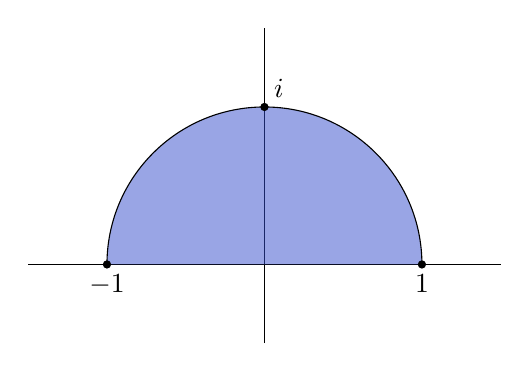
\begin{tikzpicture}
    \draw (-3, 0) -- (3, 0);
    \draw (0, -1) -- (0, 3);
    \fill [mblue, opacity=0.5] (2, 0) arc (0:180:2) -- (2, 0);
    \draw (2, 0) arc (0:180:2);
    \node [circ] at (-2, 0) {};
    \node [circ] at (2, 0) {};
    \node [circ] at (0, 2) {};
    \node at (-2, 0) [below] {$-1$};
    \node at (2, 0) [below] {$1$};
    \node at (0, 2) [anchor = south west] {$i$};
  \end{tikzpicture}
\end{center}
can be given by
\[
  \mathcal{U} = \left\{z: \arg\left(\frac{z - 1}{z + 1}\right) \in \left[\frac{\pi}{2}, \pi\right]\right\}.
\]
Thus for instance the map
\[
  z \mapsto -\left(\frac{z - 1}{z + 1}\right)^2
\]
is a conformal equivalence from $\mathcal{U}$ to $\H$. This is since $z \mapsto \frac{z - 1}{z + 1}$ maps the disk to the upper half plane, and hence $\mathcal{U}$ to the top-left quadrant. Squaring doubles the angle and gives the lower half-plane, and multiplying by $-1$ gives the upper half plane.
\begin{center}
  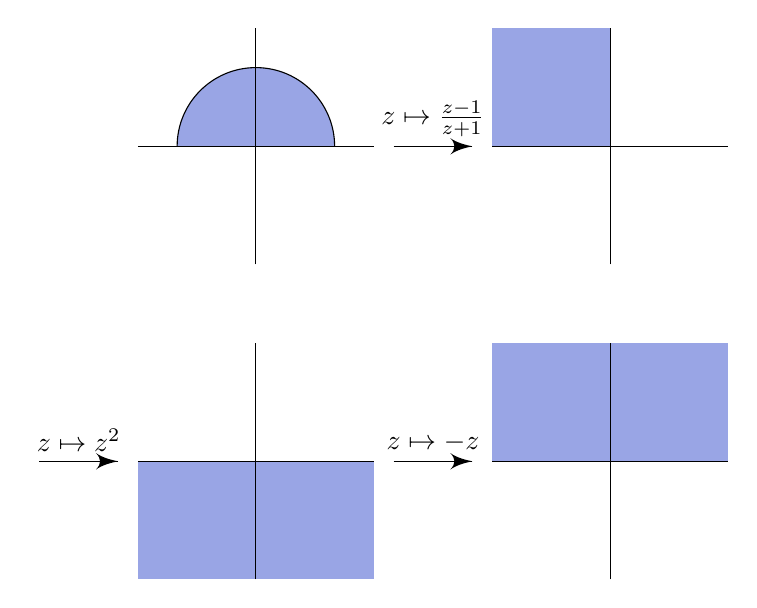
\begin{tikzpicture}[scale=0.5]
    \fill [mblue, opacity=0.5] (2, 0) arc (0:180:2) -- (2, 0);
    \draw (2, 0) arc (0:180:2);
    \draw (-3, 0) -- (3, 0);
    \draw (0, -3) -- (0, 3);

    \draw [->] (3.5, 0) -- (5.5, 0) node [pos=0.5, above] {$z \mapsto \frac{z - 1}{z + 1}$};
    \begin{scope}[shift={(9,0)}]
      \fill [mblue, opacity=0.5] (-3, 3) rectangle (0, 0);
      \draw (-3, 0) -- (3, 0);
      \draw (0, -3) -- (0, 3);

    \end{scope}
    \begin{scope}[shift={(0,-8)}]
      \draw [->] (-5.5, 0) -- (-3.5, 0) node [pos=0.5, above] {$z \mapsto z^2$};

      \fill [mblue, opacity=0.5] (-3, 0) rectangle (3, -3);
      \draw (-3, 0) -- (3, 0);
      \draw (0, -3) -- (0, 3);

      \draw [->] (3.5, 0) -- (5.5, 0) node [pos=0.5, above] {$z \mapsto -z$};
    \end{scope}
    \begin{scope}[shift={(9,-8)}]
      \fill [mblue, opacity=0.5] (-3, 0) rectangle (3, 3);
      \draw (-3, 0) -- (3, 0);
      \draw (0, -3) -- (0, 3);
    \end{scope}
  \end{tikzpicture}
\end{center}
In fact, there is a really powerful theorem telling us most things are conformally equivalent to the unit disk.

\begin{thm}[Riemann mapping theorem]
  Let $\mathcal{U} \subseteq \C$ be the bounded domain enclosed by a simple closed curve, or more generally any simply connected domain not equal to all of $\C$. Then $\mathcal{U}$ is conformally equivalent to $D = \{z: |z| < 1\} \subseteq \C\}$.
\end{thm}
This in particular tells us any two simply connected domains are conformally equivalent.

\begin{defi}[Simple closed curve]
  A \emph{simple closed curve} is the image of an injective map $S^1 \to \C$.
\end{defi}
It should be clear (though not trivial to prove) that a simple closed curve separates $\C$ into a bounded part and an unbounded part.

The more general statement requires the following definition:
\begin{defi}[Simply connected]
  A domain $\mathcal{U}\subseteq \C$ is \emph{simply connected} if every continuous map from the circle $f: S^1 \to \mathcal{U}$ can be extended to a continuous map from the disk $F: \overline{D^2} \to \mathcal{U}$ such that$F|_{\partial \overline{D^2}} = f$. Alternatively, any loop can be continuously shrunk to a point.
\end{defi}

\begin{eg}
  The unit disk is simply-connected, but the region defined by $1 < |z| < 2$ is not, since the circle $|z| = 1.5$ cannot be extended to a map from a disk.
  \begin{center}
    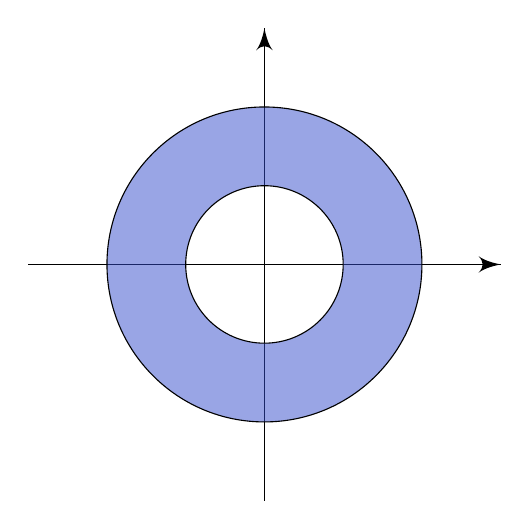
\begin{tikzpicture}
      \draw [->] (-3, 0) -- (3, 0);
      \draw [->] (0, -3) -- (0, 3);
      \fill [mblue, opacity=0.5] circle [radius=2];
      \fill [white] circle [radius=1];
      \draw circle [radius=1];
      \draw circle [radius=2];
      \draw (-1, 0) -- (1, 0);
      \draw (0, -1) -- (0, 1);
    \end{tikzpicture}
  \end{center}
\end{eg}
We will not prove this statement, but it is nice to know that this is true.

If we believe that the unit disk is relatively simple, then since all simply connected regions are conformally equivalent to the disk, all simply connected domains are boring. This suggests we will later encounter domains with holes to make the course interesting. This is in fact true, and we will study these holes in depth later.

\begin{eg}
  The exponential function
  \[
    e^z = 1 + z + \frac{z^2}{2!} + \frac{z^3}{3!} + \cdots
  \]
  defines a function $\C \to \C^*$. In fact it is conformal mapping. This sends the region $\{z: \Re(z): [a, b]\}$ to the annulus $\{e^a \leq |w| \leq e^b\}$. One is simply connected, but the other is not --- this is not a problem since $e^z$ is \emph{not} bijective on the strip.
  \begin{center}
    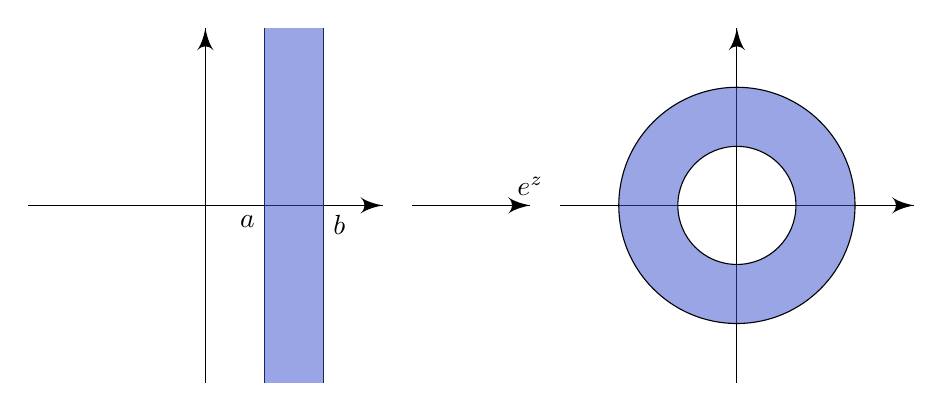
\begin{tikzpicture}[scale=0.75]
      \draw [->] (-3, 0) -- (3, 0);
      \draw [->] (0, -3) -- (0, 3);

      \draw (1, 3) -- (1, -3);
      \draw (2, 3) -- (2, -3);
      \fill [mblue, opacity=0.5] (1, 3) rectangle (2, -3);
      \node [anchor=north east] at (1, 0) {$a$};
      \node [anchor=north west] at (2, 0) {$b$};

      \draw [->] (3.5, 0) -- (5.5, 0) node [above] {$e^z$};
      \begin{scope}[shift={(9, 0)}]
        \draw [->] (-3, 0) -- (3, 0);
        \draw [->] (0, -3) -- (0, 3);
        \fill [mblue, opacity=0.5] circle [radius=2];
        \fill [white] circle [radius=1];
        \draw circle [radius=1];
        \draw circle [radius=2];
        \draw (-1, 0) -- (1, 0);
        \draw (0, -1) -- (0, 1);
      \end{scope}
    \end{tikzpicture}
  \end{center}
\end{eg}

At this point, we need to recall some facts from IB Analysis II.
\begin{defi}[Uniform convergence]
  A sequence $(f_n)$ of functions \emph{converge uniformly} to $f$ if for all $\varepsilon > 0$, there is some $N$ such that $n > N$ implies $|f_n(z) - f(z)| < \varepsilon$ for all $z$.
\end{defi}

\begin{prop}
  The uniform limit of continuous functions is continuous.
\end{prop}

We also had the following nice test for uniform convergence of a series:
\begin{prop}[Weierstrass M-test]
  For a sequence of functions $f_n$, if we can find $(M_n) \subseteq \R_{>0}$ such that $|f_n(x)| < M_n$ for all $x$ in the domain, then $\sum M_n$ converges implies $\sum f_n(x)$ converges uniformly on the domain.
\end{prop}

Finally, we have the following result.
\begin{prop}
  Given any constants $\{c_n\}_{n \geq 0} \subseteq \C$, there is a unique $R \in [0, \infty]$ such that the series $z \mapsto \sum_{n = 0}^\infty c_n(z - a)^n$ converges absolutely if $|z - a| < R$ and diverges if $|z - a| > R$. Moreover, if $0 < r < R$, then the series converges uniformly on $|z| < r$.
\end{prop}
So while we don't necessarily get uniform convergence on the whole domain, we get uniform convergence on all compact subsets of the domain.

\end{document}
